\documentclass[11pt]{article}

\usepackage{graphicx, subcaption, amsfonts, amsmath, amsthm, empheq,
  setspace, lscape}
\usepackage[top=1in, bottom=1in, left=1in, right=1in]{geometry}

% define some commands
% command to box formula
\newcommand*\widefbox[1]{\fbox{\hspace{2em}#1\hspace{2em}}}
\newlength\dlf
\newcommand\alignedbox[2]{
  % Argument #1 = before & if there were no box (lhs)
  % Argument #2 = after & if there were no box (rhs)
  &  % Alignment sign of the line
  {
    \settowidth\dlf{$\displaystyle #1$}  
    % The width of \dlf is the width of the lhs, with a displaystyle font
    \addtolength\dlf{\fboxsep+\fboxrule}  
    % Add to it the distance to the box, and the width of the line of the box
    \hspace{-\dlf}  
    % Move everything dlf units to the left, so that & #1 #2 is aligned under #1 & #2
    \boxed{#1 #2}
    % Put a box around lhs and rhs
  }
}

\newcommand{\ps}{\mathrm{\Theta}}
\newcommand{\p}{\theta}
\newcommand{\eps}{\varepsilon}
\newcommand{\be}{\begin{equation}}
\newcommand{\ee}{\end{equation}}
\newcommand\ER{Erd\H{o}s-R'{e}nyi}
\newcommand{\Forall}{\; \forall \;}
\DeclareMathOperator*{\argmin}{\arg\!\min}

% change captions
\captionsetup{width=0.8\textwidth}
% \captionsetup{labelformat=empty,labelsep=none} 

% set paragraph indent length
\setlength\parindent{0pt}

% set folder for imported graphics
\graphicspath{ {../figs/temp/} }

\title{New figures}

\begin{document}
\maketitle

\section{Singularly perturbed}

\subsection{Singularly perturbed ODE, sloppy initial conditions}

The system takes the form

\be
\begin{array}{rcl}
 \dot{x} &=& y - \lambda x ,
\vspace*{1mm}\\
 \eps \dot{y} &=& \eps x - \displaystyle\left(1+\frac{10}{1.5-\sin y}\right) y ,
\end{array}
\ \mbox{supplemented with} \
\begin{array}{rcl}
 x(0) &=& x_0 ,
\vspace*{1mm}\\
 y(0) &=& y_0 .
\end{array}
\label{elem-ODE}
\ee

The following level set plots show that at large values of $1/\epsilon$, the range of acceptable $y_0$ values increases. However, close enough to the point of interest, level sets remain ellipsoids as expected.

\begin{figure}[ht!]
    \centering
    \includegraphics[width=\textwidth]{model-manifold-eps-coloring-small-eps}
    \caption{Plain model manifold colored by $1/\epsilon$}
\end{figure} %
\begin{figure}[ht!]
    \centering
    \includegraphics[width=\textwidth]{model-manifold-y0-coloring-small-eps}
    \caption{Plain model manifold colored by $y_0$}
\end{figure} %

Now we plot the $\delta$-ball around the point $y_0 = 5$, $1/\epsilon = 100$, both in parameter space and model space.

\begin{figure}[ht!]
    \centering
    \includegraphics[width=\textwidth]{levelsets-small-eps}
    \caption{Boundaries of the $\delta$-ball plotted in parameter space, for increasing values of $\delta$.}
\end{figure}
\begin{figure}[ht!]
    \centering
    \includegraphics[width=\textwidth]{model-manifold-ball-small-eps}
    \caption{Largest $\delta$-ball in model space. Note how it envelopes the corner of the manifold, suggesting an unbounded boundary in parameter space.}
\end{figure}


If we move the ball to a different location on the model manifold, the boundaries change dramatically as the system no longer exhibits sloppiness. First we look at the plain model manifold.

\begin{figure}[ht!]
    \centering
    \includegraphics[width=\textwidth]{model-manifold-eps-coloring-medium-eps}
    \caption{Plain model manifold colored by $1/\epsilon$}
\end{figure} %
\begin{figure}[ht!]
    \centering
    \includegraphics[width=\textwidth]{model-manifold-y0-coloring-medium-eps}
    \caption{Plain model manifold colored by $y_0$}
\end{figure} %

Now we plot the $\delta$-ball around the point $y_0 = 5$, $1/\epsilon = 3$, both in parameter space and model space.

\begin{figure}[ht!]
    \centering
    \includegraphics[width=\textwidth]{levelsets-medium-eps}
    \caption{Boundaries of the $\delta$-ball plotted in parameter space, for increasing values of $\delta$.}
\end{figure}
\begin{figure}[ht!]
    \centering
    \includegraphics[width=\textwidth]{model-manifold-ball-coloring-medium-eps}
    \caption{Largest $\delta$-ball in model space. Note how it envelopes the corner of the manifold, suggesting an unbounded boundary in parameter space.}
\end{figure}

\subsection{ABC Reaction}

The mechanism is given by

\begin{align*}
  A \xrightleftharpoons[k_{-1}]{k_1} B, \; B \xrightarrow[]{k_2} C
\end{align*}

which, under the QSSA, gives a $k_{eff}$ of

\begin{align*}
  k_{eff} = \frac{k_1 k_2}{k_{-1} + k_2}
\end{align*}

Thus, we expect a nonlinear neutral set. Below we plot the neutral sets in parameter space showing the nonlinear character of $k_{eff}$. As we increase $\delta$ in the second figure, we begin to see generic three-dimensional dependence on the base parameters.

\begin{figure}[ht!]
    \centering
    \includegraphics[width=\linewidth]{./keff-small-delta}
\end{figure}
\begin{figure}[ht!]
    \centering
    \includegraphics[width=\linewidth]{./keff-large-delta}
  \end{figure} %



%% \begin{figure}[htbp]
%%   \centering
%%   \caption{Dataset of sloppy parameter combinations overlayed with
%%     with a surface of $k_{eff} =0.502$. All points satisfy $c(\theta)
%%     \le 10^{-6}$.}
%% \end{figure}

%% As expected, it maps out a two-dimensional surface in parameter space over which $k_{eff}$ is nearly constant ($k_{eff} \in (0.4, 1.0)$ in the dataset above).

%% When DMAPS was applied, the first two eigenvectors parameterized the surface as hoped. This is shown in the two figures below.

%% % \begin{figure}[htbp]
%% %   \centering
%% %   \includegraphics[width=\linewidth]{abc-dmap1}
%% %   \caption{Coloring the dataset by the first DMAP parameter/coordinate value}
%% % \end{figure}

%% % \begin{figure}[htbp]
%% %   \centering
%% %   \includegraphics[width=\linewidth]{abc-dmap2}
%% %   \caption{Coloring the dataset by the second DMAP parameter/coordinate value}
%% % \end{figure}

%% Additionally, we can use the mixed DMAPS kernel to find the important
%% parameter $k_{eff}$ if we apply it to a dataset arising from a larger
%% ball in model space (which can also be thought of as increasing the
%% tolerance of our fitting routine). Fig. \ref{fig:dmaps-mixed} shows
%% that the third eigenvector maps to $k_{eff}$.

%% \begin{figure}[htbp]
%%   \centering
%%   \includegraphics[width=\linewidth]{./rawlings/3d-dmaps}
%%   \caption{Coloring the enlarged parameter set by $k_{eff}$ (top
%%     right) and by the third DMAPS eigenvector (bottom right). The
%%     colors are similar in both, suggesting the third eigenvector is
%%     one-to-one with $k_{eff}$. \label{fig:dmaps-mixed}}
%% \end{figure}

%% \subsection{The singular regime}

%% Ideally, we would operate where $k_2 \gg k_1, \; k_{-1}$. However,
%% limiting our analysis to this region leads to

%% \begin{align*}
%%   k_{eff} &= \frac{k_1}{\frac{k_{-1}}{k_2} + 1}
%%   & \approx k_1
%% \end{align*}

%% which removes the nonlinearity from the contours. If we could ease our
%% restrictions to just $k_2 \gg k_1$ we do recover the desired curvature.


%% \section{Regularly perturbed}

%% Here we have the Michaelis Menten system. Although it, too, is singularly perturbed, the parameter transformation we apply reveals two \textit{regular} perturbation paramters $\kappa$ and $\epsilon$.

%% \subsection{Michaelis Menten}

%% This reaction system is given by
%% %
%% \[
%%  {\rm S + E}
%% \
%%  \xrightleftharpoons[k_{-1}]{k_1}
%% \
%%  {\rm C}
%% \
%%  \xrightarrow{k_2}
%% \
%%  {\rm P + E} ,
%% \label{s2c2p}
%% \]
%% %

%% The initial constituent concentrations are
%% %
%% \be
%%  S(0) = S_0 ,
%% \quad
%%  E(0) = E_0 ,
%% \quad
%%  C(0) = C_0
%% \quad\mbox{and}\quad
%%  P(0) = P_0 ,
%% \label{SCEP-IC}
%% \ee
%% %
%% and they supplement the ODEs governing the evolution
%% of the constituent concentrations,
%% %
%% \be
%% \begin{array}{rclcl}
%%  S' &=& -k_1 E S + k_{-1} C ,
%% \\
%%  C' &=& \ \ \, k_1 E S - (k_{-1} + k_2) C ,
%% \\
%%  E' &=& -k_1 E S + (k_{-1} + k_2) C ,
%% \\
%%  P' &=& \ \ \, k_2 C .
%% \end{array}
%% \ee

%% System~\eqref{SCEP-IC}--\eqref{SCEP-ODE} has
%% two exact conservation laws expressing mass balance,
%% %
%% \[
%%  S+C+P = S_0+C_0+P_0 =: S_T
%% \quad\mbox{and}\quad
%%  C+E = C_0+E_0 =: E_T .
%% \]
%% %
%% These may be employed to eliminate two of the ODEs;
%% these are traditionally chosen to be
%% the equations for $E$ and $P$,
%% so that
%% %
%% \be
%% \begin{array}{rclcl}
%%  S' &=& -k_1 (E_T-C) S + k_{-1} C ,
%% \\
%%  C' &=& \ \ \, k_1 (E_T-C) S - (k_{-1} + k_2) C .
%% \end{array}
%% \label{SC-ODE}
%% \ee
%% In a typical experimental setting,
%% both $C_0$ and $P_0$ equal zero,
%% so that $S_0$ and $E_0$ fully determine $S_T$ and $E_T$,
%% %
%% \be
%%  S_0 = S_T
%% \quad\mbox{and}\quad
%%  C_0 = 0 .
%% \label{SC-IP}
%% \ee
%% %
%% We will follow this convention here and consider a problem with five
%% parameters: the three kinetic constants $k_{-1}$, $k_1$ and $k_2$, on
%% one hand, and the total concentrations $S_T$ and $E_T$ on the other. \\

%% Next we transform the bare parameters into 

%% \begin{align*}
%%   V_M &= k_2 E_T \\
%%   K_M &= \frac{k_{-1} + k_2}{k_1} \\
%%   \kappa &= \frac{k_{-1}}{k_2} \\
%%   \epsilon &= \frac{E_T}{S_T + K_M} \\
%% \end{align*}

%% in which $\kappa$ and $\epsilon$ drop out of the leading dynamics and are thus sloppy. However, these parameter combinations \textbf{do not} yield nonlinear contours in the original parameter space as desired. The figure below shows the ellipsoidal contour produced by this system in the $K_M$, $V_M$ and $S_T$ parameter space, combinations of which are also sloppy in certain regimes.

%% \begin{figure}[htbp]
%%   \centering
%%   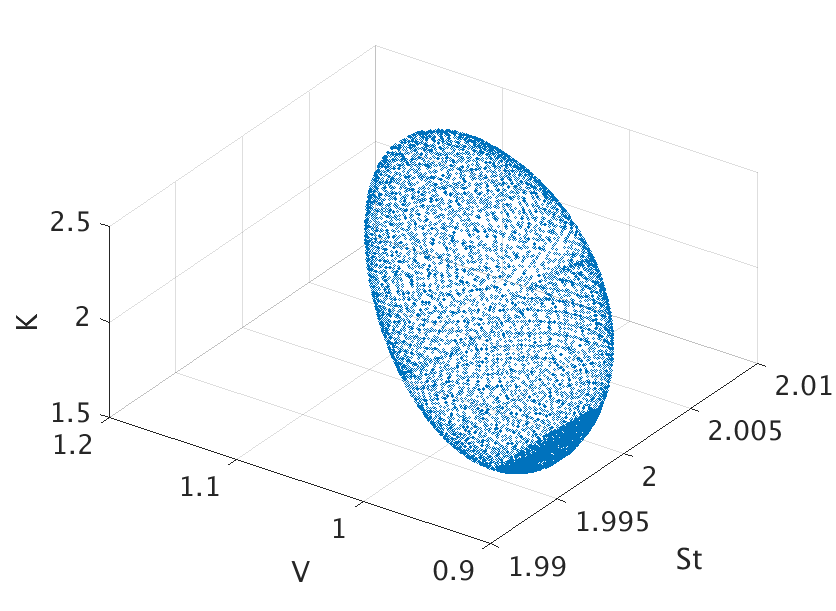
\includegraphics[width=\linewidth]{./zagaris/k-v-st-contour}
%%   \caption{Ellipsoidal contour of Michaelis Menten system in $K_M$, $V_M$ and $S_T$ parameter space.}
%% \end{figure}

%% \section{Singularly and regularly perturbed}

%% Here we turn to Antonios' model which includes all varieties of sloppiness we wish to show: singular and regular perturbation parameters and sloppy initial conditions. This system is ideal for a nonlinear transformation of parameters.

%% \subsection{Antonios' Model}

%% We start with the linear ODEs

%% \begin{align*}
%%   X &= -\lambda X \\
%%   \epsilon Y &= -Y
%% \end{align*}

%% and then transform it into nonlinear $(x, y)$ via 

%% \begin{align*}
%%   x &= X + \phi(y) \\
%%   y &= Y + \mu(x) \\
%% \end{align*}

%% We are free to choose $\phi(y)$ and $\mu(x)$, which control the shape of the fast and slow manifold, respectively. Thus, if we set $\mu = a x^2$ and $\phi = b y^2$ we find parabolic slow and fast manifolds, and additionally we've introduced a sloppy regular perturbation parameter $b$. Additionally, initial conditions lying along a given fast manifold will be sloppy. Sloppiness in $\epsilon$/$\lambda$, $a$/$b$ and $x_0$/$y_0$ are shown in the three figures below.

%% \begin{figure}[htbp]
%%   \centering
%%   \includegraphics[width=\linewidth]{./zagaris/sing-pert-init-cond-contours}
%%   \caption{$x_0$/$y_0$ plane colored by objective function value. The contours follow the fast manifold $x=y^2$.}
%% \end{figure}

%% \begin{figure}[htbp]
%%   \centering
%%   \includegraphics[width=\linewidth]{./zagaris/sing-pert-phase-plane}
%%   \caption{The phase plane showing parabolic fast and slow
%%     trajectories on their approach to the stable steady state at the origin.}
%% \end{figure}


%% \subsubsection{Nonlinear parameter transformation}

%% By holding the sloppy parameters $(\epsilon, b)$ constant we are left
%% with a system in which both remaining parameters, $\lambda$ and $a$
%% are not sloppy. If we apply two iterations of the H\'{e}non map to a
%% set of $(\lambda, a)$ values that fit some base model within a given
%% tolerance, we can make the transformed parameters $(\theta_1,
%% \theta_2)$ appear sloppy.

%% \begin{figure}[ht!]
%%   \begin{subfigure}[t]{0.49\textwidth}
%%     \centering
%%     \includegraphics[width=\textwidth]{./transformed-params/transformed-params-fromoptimization-insert}
%%     \subcaption{Parameter values found through repeated fitting of
%%       the model with parameters transformed via the H\`{e}non map. \label{f.henon}}
%%   \end{subfigure}
%%   \begin{subfigure}[t]{0.49\textwidth}
%%     \centering
%%     \includegraphics[width=\textwidth]{./transformed-params/inverted-params}
%%     \subcaption{Original parameter values found by inverting the
%%       collection in the left panel.  \label{f.henon-inverse}}
%%   \end{subfigure} %
%%   \caption{The set $\ps_\delta$ corresponding to the point
%%     $(\alpha_*,\lambda_*) = (1,1)$. The absence of
%%     sloppiness is evident in the right panel, in which $\ps_\delta$ is
%%     plotted in terms of the original parameter set
%%     $(\alpha,\lambda)$. To the contrary, the same domain plotted in
%%     terms of the transformed parameters $(\p_1,\p_2)$ appears bent and
%%     sloppy. \label{f.transf-params}}
%% \end{figure}

%% \subsubsection{Two effective parameters, one neutral}

%% We can also hold $b$ constant to obtain a model with two effective
%% parameters $\lambda$ and $a$, and one neutral, $\epsilon$. This gives
%% us another context in which we can demonstrate the advantage the mixed DMAPS
%% kernel offers over the standard gaussian. Here, we uncover both
%% effective parameters $\lambda$ and $a$ in the first two DMAPS
%% eigenvectors despite the much larger variation in $\eps$. This kernel
%% is given by

%% \begin{align*}
%%   k(\theta_i, \theta_j) = \exp(- \frac{\|\theta_i -
%%   \theta_j\|^2}{\eps}  - \frac{\|f(\theta_i) - f(\theta_j)\|^2}{\eps^2})
%% \end{align*}

%% The results of applying this variant of DMAPS to a set of $(\lambda,
%% a, \eps)$ parameters is shown below.


%% \begin{figure}[ht!]
%%   \begin{subfigure}[t]{0.49\textwidth}
%%     \centering
%%     \includegraphics[width=\textwidth]{./two-effective-one-neutral/dmaps-phi1}
%%     \subcaption{Coloring sloppy parameter combinations by $\Phi_1$}
%%   \end{subfigure}
%%   \begin{subfigure}[t]{0.49\textwidth}
%%     \centering
%%     \includegraphics[width=\textwidth]{./two-effective-one-neutral/dmaps-phi2}
%%     \subcaption{Coloring sloppy parameter combinations by $\Phi_2$}
%%   \end{subfigure} %
%%   \caption{The set $\ps_\delta$ corresponding to the point
%%     $(\alpha_*,\lambda_*) = (1,1)$. The absence of
%%     sloppiness is evident in the right panel, in which $\ps_\delta$ is
%%     plotted in terms of the original parameter set
%%     $(\alpha,\lambda)$. To the contrary, the same domain plotted in
%%     terms of the transformed parameters $(\p_1,\p_2)$ appears bent and
%%     sloppy. \label{f.transf-params}}
%% \end{figure}

% \bibliographystyle{plain}
% \bibliography{literature.bib}

\end{document}
